\documentclass[a4paper]{article}
\usepackage{lipsum}
\usepackage{url}
\usepackage{graphicx}
\usepackage{listings}
\lstset{language=Python}
\usepackage[margin=2cm]{geometry}
\usepackage{indentfirst}
\usepackage{xcolor}
\usepackage{lmodern}
\usepackage{enumitem}
\renewcommand{\familydefault}{\sfdefault}
\graphicspath{ {images/} }

\begin{document}

% TODO: Anything else needed for titlepage
\begin{titlepage}
	\newcommand{\HRule}{\rule{\linewidth}{0.5mm}}
	\center{}

    %Headings
	\LARGE{University of Nottingham}\\[1.5cm]
	\Large{Computer Science with Artificial Intelligence MSci}\\[0.5cm]
	\large{G54IRP/COMP4027 - Individual Research Project}\\[0.5cm]

    %Title
	\HRule{}\\[0.4cm]
	{\huge\bfseries AI for General Video Game Playing}\\[0.4cm]
	\HRule{}\\[1.5cm]

    %Authors
	\begin{minipage}{0.4\textwidth}
		\begin{flushleft}
			\large
			\textit{Author}\\
			Benjamin Charlton\\
            psybc3@nottingham.ac.uk\\
            4262648
		\end{flushleft}
	\end{minipage}
    \begin{minipage}{0.4\textwidth}
		\begin{flushright}
			\large
			\textit{Supervisor}\\
			Dr.\@ Ender \"Ozcan\\
            Ender.Ozcan@nottingham.ac.uk
		\end{flushright}
	\end{minipage}

    %Date
	\vfill\vfill\vfill
	{\large7\textsuperscript{th} December 2017}
	\vfill

\end{titlepage}

%Contents Page
\pagenumbering{roman}
\tableofcontents
\pagebreak

\pagenumbering{arabic}
\section{Introduction}
\subsection{Introduction}
\begin{itemize}
    \item Popularity of Video Games
    \item Variety of Video games being played
    \item Video Games as a testing ground for AI
\end{itemize}
\subsection{Planning VS learning}
\begin{itemize}
    \item As the title says, just to get some definitions out of the way
\end{itemize}
\subsection{Motivation}
\begin{itemize}
    \item Individual desire to get better at deep reinforcement learning
    \item Learning more Methods
    \item Applying Methods
    \item Learning to use more robust and real world frameworks for DRL \\
    \item Seeing the state of the art in DRL and AI game playing
\end{itemize}
\subsection{Aims and Objectives}
\begin{itemize}
    \item Look at the project plan aims and objectives
\end{itemize}

\section{Related Work}
\subsection{AI and Game Playing}
\begin{itemize}
    \item AI approaches have specialised heuristics or only been developed for a single game
    \\
    \item Go - previous interim report / PP
    \item Chess - previous interim report / PP
    \item OpenAIFive
    \item GET MORE THINGS FROM PP
    \\
    \item Dartmouth Workshop
\end{itemize}

\subsubsection{Early Artificial Intelligence}
%TODO: Maybe extend / re sort this section
The history of AI game playing begins near the start of artificial intelligence as a field, in the 1950s.
Strachey created a draughts player for one of the first general computing machines (Manchester Ferranti Mark I) which by  1952 could ``play a complete game of draughts at a reasonable speed''\cite{BreifHistoryComputing}.
Prinz wrote a simplified chess player for the Manchester Machine as well which could solve the mate-in-two problem.
This meant that if there was a checkmate solution in 2 turns it could successfully find it\cite{BreifHistoryComputing}.
Prinz simply used an exhaustive search technique to find the correct moves, and even though computing power was limited at the time it was clear that this wouldn't scale to full games.
This lead to Turning starting to program `Turbochamp' a chess program that would be able to play a full game of chess using heuristics\cite{BreifHistoryComputing}
\par
These simple games were made before the term artificial intelligence was being used even in an academic setting showing how natural AI and game playing go together.

\subsubsection{Chess}
Chess was an early and significant example in the history of AI game playing.
In 1997 IBM managed to beat the reigning world champion, Garry Kasparov, using their custom developed machine, Deep Blue\cite{deepBlue}.
This was significant as, at the time, creating a winning chess AI was seen to be the next big milestone at the time in AI\@.
\par
To achieve this Deep Blue used a combination of techniques with the main underlying AI technique being a search method.
As Chess is a deterministic game and both players have complete information of the board state it was possible for Deep Blue to generate future board states.
With this forward model its possible to generate a search tree of possible moves and their resulting game states
The tree was efficiently generated by a combination of a massively parallel architecture over 30 nodes and the fact that each node has special purpose chess chips, generating around 6--8 moves ahead on average.
Alpha-beta pruning was used in a MinMax algorithm to help efficiently search the tree while using the custom hardware to evaluate each node quickly.
\par
IBM had proven that search methods could achieve strong results against human opponents but this was mostly due to brute force computing power and a heavy reliance on expert knowledge.
The expert knowledge came from other grandmasters and was used in the form of an opening/closing move database and the special purpose hardware to evaluate board states.
While higher computing power will always benefit AI techniques, later techniques have been developed to reduce the need of expert knowledge and to make more efficient use of hardware available.

\subsubsection{Go}


\subsection{GVGAI and VGDL}
\begin{itemize}
    \item TODO Make some notes up here
\end{itemize}
\subsection{OPEN AI GYM and GVGAI GYM}
\begin{itemize}
    \item What is OPEN AI GYM
    \item Why is OPEN AI GYM helpful for RL
    \item GVGAI GYM
    \item Initial results from GVG AI GYM paper
    \item Maybe some more here :)
\end{itemize}
\cite{GVGAIGYM}
\subsection{Subsection to end all subsections}
\begin{itemize}
    \item Maybe something about the open AI baselines
    \item Depends what technique I would be using but I should look into that
    \item Where does reinforcement learning come into this bad buoy
\end{itemize}


\pagebreak
\section{Appendix}

\subsection{Meeting Minutes}


\pagebreak
\subsection{Work Plan}
% \begin{center}
    % 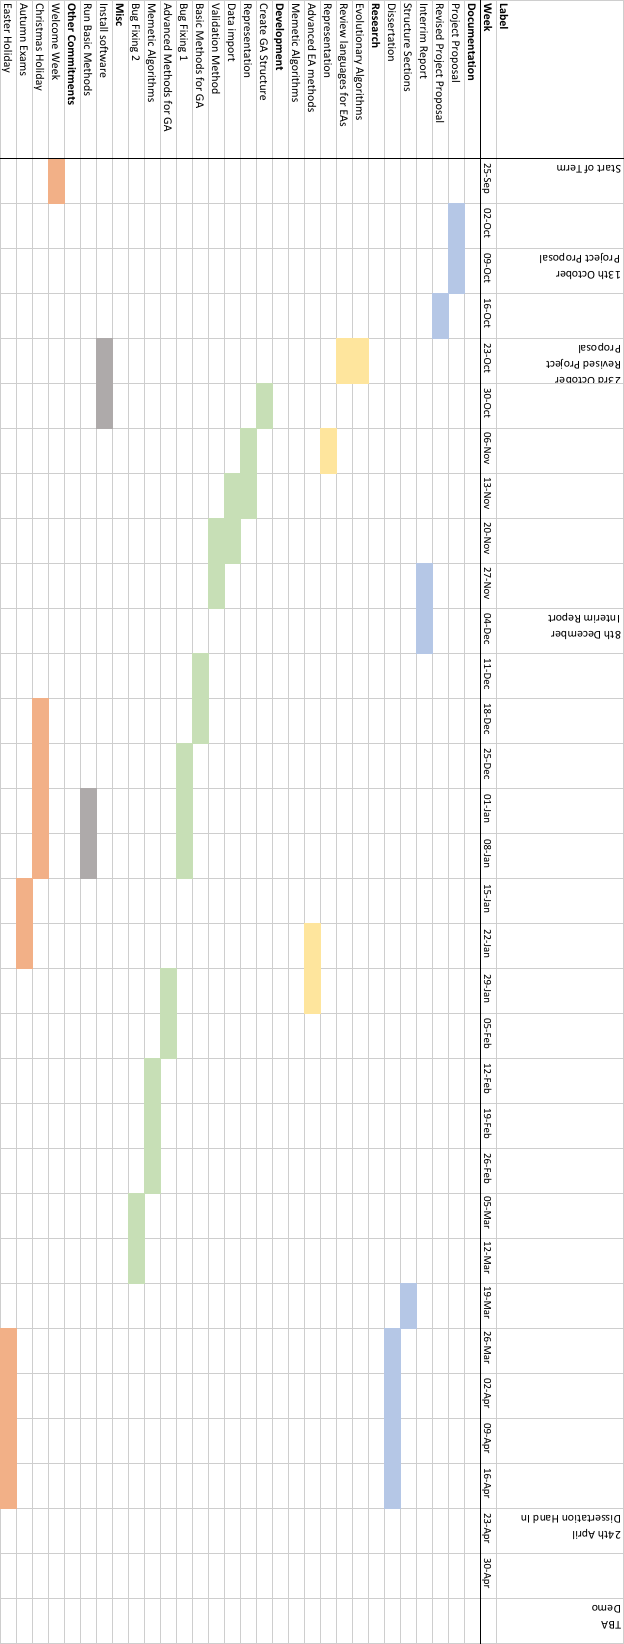
\includegraphics[height=24.8cm]{workPlan.png}
% \end{center}


%Bibliography
\subsection{References}
\bibliography{InterimReport}
\bibliographystyle{plain}


\end{document}
